%
\hsection{\crowsFoot{G}{O1}{H}{MM}}%
\label{sec:rm:gh}%
%
\begin{figure}%
\centering%
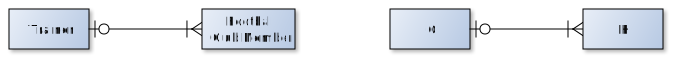
\includegraphics[width=0.97\linewidth]{\currentDir/GH}%
\caption{An example of the \crowsFoot{G}{O1}{H}{MM} relationship pattern from back in \dref{sec:conceptual:relationshipCardinalities}.}%
\label{fig:rm:gh}%
\end{figure}%
%
\gitSQLAndOutput{\databasesCodeRepo}{conceptualToRelational}{GH_tables.sql}{relationships}{}{}{postgres.sh}{GH_tables}{%
The realization of an \crowsFoot{G}{O1}{H}{MM} conceptual relationship.%
}%
%
\gitSQLAndOutput{\databasesCodeRepo}{conceptualToRelational}{GH_insert_and_select.sql}{relationships}{}{}{postgres.sh}{GH_insert_and_select}{%
Inserting into and selecting data from the realization of an \crowsFoot{G}{O1}{H}{MM} conceptual relationship given in \cref{lst:GH_tables}.%
}%
%
\gitExec{cdtrmTableG}{\databasesCodeRepo}{conceptualToRelational}{../_scripts_/db_table_to_latex_table.sh relationships g gid;fkhid;x}%
\gitExec{cdtrmTableH}{\databasesCodeRepo}{conceptualToRelational}{../_scripts_/db_table_to_latex_table.sh relationships h hid;fkgid;y}%
%
\begin{figure}%
\centering%
\floatSep%
\input{\gitFile{cdtrmTableG}}%
\floatSep%
\input{\gitFile{cdtrmTableH}}%
\floatSep%
\caption{The contents of the the two tables in the implementation of the \crowsFoot{G}{O1}{H}{MM} conceptual relationship after executing \cref{lst:GH_insert_and_select}.}%
\label{fig:rm:gh:tables}%
\end{figure}%
%
\gitSQLAndOutput{\databasesCodeRepo}{conceptualToRelational}{GH_insert_error_1.sql}{relationships}{}{}{postgres.sh}{GH_insert_error_1}{%
Trying to create a row into table~\sqlil{g} that is not related to any row in table~\sqlil{h} is not possible.%
}%
%
\gitSQLAndOutput{\databasesCodeRepo}{conceptualToRelational}{GH_insert_error_2.sql}{relationships}{}{}{postgres.sh}{GH_insert_error_2}{%
Trying to create a row in table~\sqlil{g} that references a row in table~\sqlil{h} which is not referencing any row in table~\sqlil{g} is not possible.%
}%
%
\gitSQLAndOutput{\databasesCodeRepo}{conceptualToRelational}{GH_insert_error_3.sql}{relationships}{}{}{postgres.sh}{GH_insert_error_3}{%
Trying to create a row in table~\sqlil{g} that references a row in table~\sqlil{h} which is already referencing another row in table~\sqlil{g} is not possible.%
}%
%
\gitSQLAndOutput{\databasesCodeRepo}{conceptualToRelational}{GH_insert_error_4.sql}{relationships}{}{}{postgres.sh}{GH_insert_error_4}{%
Trying the same thing as in \cref{lst:GH_insert_error_3}, but this time also attempting to re-adjusting the row in~\sqlil{h} with an~\sqlil{UPDATE} instruction to make it reference the new row in table~\sqlil{g}, is also not possible.%
}%
%
\gitSQLAndOutput{\databasesCodeRepo}{conceptualToRelational}{GH_insert_error_5.sql}{relationships}{}{}{postgres.sh}{GH_insert_error_5}{%
Changing a row in table~\sqlil{h} that references a row in table~\sqlil{g} to now reference another row in table~\sqlil{g} is not possible.%
}%
%
We have the two entity types~G and~H.
Each entity of type~G must be connected to at least one but maybe many entities of type~H.
Each entity of type~H is connected to zero or one entity of type~G.

An example of the \crowsFoot{G}{O1}{H}{MM} relationship pattern is given back in \dref{sec:conceptual:relationshipCardinalities}:
In a soccer club, each trainer coaches several club members.
Each member can be coached by one trainer or, if they have other functions, not be coached at all.
This example is illustrated in \cref{fig:rm:gh}.

We again create two tables~\sqlil{g} and~\sqlil{h}, respectively.
They have the primary keys~\sqlil{gid} and~\sqlil{hid} as well as the example attributes~\sqlil{x} and~\sqlil{y}, respectively.
Then we can approach this in the same way as the in the two-table manner in the \crowsFoot{E}{O1}{F}{OM} situation.
However, enforcing this relationship pattern is a bit more complicated, but doable, as illustrated in \cref{lst:GH_tables}:

We begin by preparing the table~\sqlil{g}.
Each entity of type~G must be related to at least one entity of type~H.
We solve this problem in two steps:
First, we enforce that each row in table~\sqlil{g} is connected to one row in table~\sqlil{h}.
Later, we permit that it can be connected to more rows.
We therefore begin by adding an attribute~\sqlil{fkhid}, which must be \sqlil{NOT NULL}.
This column should always point to the row in table~\sqlil{h} with the same value in~\sqlil{hid}.
We will later add a proper \sqlil{REFERENCE} constraint via~\sqlil{ALTER TABLE}, because we cannot add it yet, because table~\sqlil{h} does not yet exist.
So for now, just imagine that we had added it and that this attribute always references on row in table~\sqlil{h}.
We will consider this attribute to identify the \inQuotes{primary~H}~entity to which the row in table~\sqlil{g} is related.
We make this column also \sqlil{UNIQUE}, because no row in table~\sqlil{h} can be related to more than one row in table~\sqlil{g}.
Thus, no primary key value~\sqlil{hid} can thus occur more than once in column~\sqlil{fkhid}.

Now we prepare the table for entity type~H.
Since each entity of type~H can be related to either zero or one entity of type~G, we add a column~\sqlil{fkgid} to this table.
This column can be \sqlil{NULL}, in which case the corresponding row in~\sqlil{h} is not related to any entity of type~G.
If it is not \sqlil{NULL}, then it must be a proper foreign key reference to a row in table~\sqlil{g}.
This column does \emph{not} need to be \sqlil{UNIQUE}, as multiple entities of type~H can be related to the very same entity of type~G.%
%
\begin{sloppypar}%
At this stage, we have enforced that each entity of type~H can be related to zero or one entity of type~G.
We could now go and add a constraint~\sqlil{g_fkhid_fk} as~\sqlil{FOREIGN KEY (fkhid) REFERENCES h (hid)} to table~\sqlil{g} via~\sqlil{ALTER TABLE g ADD CONSTRAINT...}.
This would enforce that each entity of type~G must be related to at least one entity of type~H.
However, this would \emph{not} enforced that, if an entity of type~G is related to one entity of type~H as its~\inQuotes{primary~H,} then that \emph{very same} H~entity also is related to the G~entity.%
\end{sloppypar}%
%
We can do this by creating the foreign key \sqlil{REFERENCES} constraint not on the single column~\sqlil{hid}, but by enforcing that the pair~\sqlil{(fkhid, gid)} from table~\sqlil{g} must also appear as pair~\sqlil{(hid, fkgid)} in table~\sqlil{h}.
We know that each value of~\sqlil{gid} can only exist once in table~\sqlil{g}.
We also know that each value of~\sqlil{hid} can only exist once in table~\sqlil{h}.
Therefore, the first part of the column pair in the constraint, \sqlil{fkhid}~(or, looking at it from the other side,~\sqlil{hid}), already selects one unique row in table~\sqlil{h}.
There can never be another row with the same~\sqlil{hid} value, because that's the primary key of table~\sqlil{h}.
The second element of the pair, i.e.,~\sqlil{gid}~(or, looking from the other side,~\sqlil{fkgid}) thus forces that this single row in table~\sqlil{h} has the value~\sqlil{gid} stored in~\sqlil{fkgid}.
Since foreign key \sqlil{REFERENCES} constraints can only reference \sqlil{UNIQUE} column(s), we must add the constraint~\sqlil{UNIQUE (hid, fkgid)} to table~\sqlil{h}.%
%
\begin{sloppypar}%
Let's go over this one more time:
We specify the constraint~\sqlil{g_fkhid_gid_fk} as~\sqlil{FOREIGN KEY (fkhid, gid) REFERENCES h (hid, fkgid)}.
On the side of the table~\sqlil{g}, this constraint looks at a row and takes the value of its foreign key~\sqlil{fkhid} to table~\sqlil{h} together with its own primary key~\sqlil{gid} as a tuple.
On the side of the table~\sqlil{h}, there must be a corresponding tuple with the primary key~\sqlil{hid} and the value of its corresponding foreign key~\sqlil{fkgid}.
Of course, the primary keys of both tables are always unique.
Let's say a row in table~\sqlil{g} has primary key~\sqlil{gid=u} and foreign key~\sqlil{fkhid=v}.
Then the row in table~\sqlil{h} with primary key~\sqlil{hid=v} must have the foreign key~\sqlil{fkgid=u}.
Of course, there could also be another row in table~\sqlil{h} which also has foreign key~\sqlil{fkgid=u}.
That's OK, because multiple entities of type~H can reference the same entity of type~G.
\end{sloppypar}%
%
With these constraints, given in \cref{lst:GH_tables}, we have implemented the relationship pattern.
Let us check what we have done.

Can we insert a row into table~\sqlil{g} that is not related to at least one row in table~\sqlil{h}?
No, we cannot, as shown in \cref{lst:GH_insert_error_1}.
Inserting a row in~\sqlil{g} requires us to specify a value for the foreign key~\sqlil{fkhid} and the corresponding row in table~\sqlil{h} must exist.
We can insert rows into table~\sqlil{h} that are not related to any row in table~\sqlil{g}, but that is OK:
Entities of type~H are related to either zero or one entities of type~G.
But could we insert a row into table~\sqlil{G} that references a row in table~\sqlil{h} that is not already related to another entity of type~G?
No, because the constraint~\sqlil{g_fkhid_gid_fk} requires that the corresponding row in table~\sqlil{h} would reference back to the row in table~\sqlil{g}~(\cref{lst:GH_insert_error_2}).

So how do we actually insert rows into table~\sqlil{g}?
We cannot insert a row that does not references a row in table~\sqlil{h}.
We cannot insert a row that references no row in table~\sqlil{g}.
And if we wanted to insert a row into table~\sqlil{g} that references a row in table~\sqlil{h} that already references some row in table~\sqlil{g}, then this would mean that we already need to have an existing row in table~\sqlil{g}.
Which we do not have.

Now that we have created our two tables and protected their referential integrity using fierce constraints, we need to see that we can insert data into them.
We have to solve this odd chicken-and-egg problem.

In \cref{lst:GH_insert_and_select}, we begin by first filling the table~\sqlil{h}.
Since entities of type~H do not necessarily be related any entity of type~G, this can be done without worrying about constraints.
When we insert an entity of type~G into our table~\sqlil{g}, we must, at the same time, create a relationship to an entity of type~H in table~\sqlil{h}.
We do this by knowing that:%
%
\cquotation{PGDG:PD:CT2}{%
A constraint that is not deferrable will be checked immediately after every command. %
Checking of constraints that are deferrable can be postponed until the end of the transaction\dots%
}%
%
In \postgresql~(and probably several other \pglspl{dbms}), referential integrity constraints are checked at the end of a command's execution.
Indeed, a single command in \postgresql\ behave like transactions~\cite{PGDG:T}, meaning that referencial integrity constraints are checked at at the end of the command execution.
The changes are committed to the data if the constraints are met and rolled back otherwise.
To insert a row into table~\sqlil{g}, we also need to modify a record from table~\sqlil{h} that currently is unrelated to any row in~\sqlil{g} to relate to that new row,
If we can wrap the insertion and the modification into a single \sql\ command, then things might work.

In order to modify the row in table~\sqlil{h}, we must know the primary key~\sqlil{gid} of the new row in table~\sqlil{g}.
We declared the primary key~\sqlil{gid} of table~\sqlil{g} as \sqlil{INT GENERATED BY DEFAULT AS IDENTITY PRIMARY KEY}.
This means that the values of this key are generated when the rows are created.
This, in turn, means that before inserting the row into table~\sqlil{g}, we do not know the value that its primary key will have.
Luckily, this is a very common problem:~\inQuotes{What if we insert some data into a table with automatically generated primary keys and then need the key that was assigned to that data?}
\postgresql\ offers an answer with the \sqlilIdx{RETURNING} keyword\footnote{%
This is a \postgresql\ addition to~\sql~\cite{SE:DA:2020WDSSOAOTNPSDIOR} and does not seem to be part of the \sql\ standard, but it is also supported by \mariadb~\cite{M:MSD:IR} and \sqlite~\cite{HWACIS:R}.%
}~\cite{PGDG:PD:RDFMR}.%

The statement \sqlil{INSERT INTO g (fkhid, x) VALUES (1, '123') RETURNING gid, fkhid} would insert a row into the table~\sqlil{g} where the value of the attribute~\sqlil{x} is~\sqlil{'123'} and the value of the attribute~\sqlil{fkhid} is~\sqlil{1}.
It would return the value of the primary key column~\sqlil{gid} that was automatically generated and assigned to this row as well as the value of~\sqlil{fkhid}, which would be~\sqlil{1} in this case.
Of course, this statement will fail, because it would violate our constraint \sqlil{g_fkhid_gid_fk} from \cref{lst:GH_tables}.
But we are one step closer to make things work.%
%
\begin{sloppypar}%
One idea would be to build some Frankensteinian query trying to plug the first insert into the second in the
 form \sqlil{UPDATE h SET gid = (INSERT INTO g (fkhid, x) VALUES (1, '123')}\linebreak[3]\sqlil{RETURNING gid, fkhid) WHERE h.hid = fkhid;}.
This is not a valid approach in \sql, and \postgresql\ does not like this either.
It would be a single statement, but this does not work.%
\end{sloppypar}%
%
However, we can use another tool:~\glsreset{CTE}\pglspl{CTE}.
A~\pgls{CTE} allows us to assign a name to a sub-expression of a query.
This sub-expression then works a bit like a temporary table.
It is evaluated only once and can be used like a read-only table in other queries.
For example, \sqlil{WITH cats AS (SELECT age, name FROM animals WHERE type='cat')}\sqlIdx{WITH}, we would assign the result of the query \sqlil{SELECT age, name FROM animals WHERE type='cat'} to the \pgls{CTE}~\sqlil{cats}.
We could then use \sqlil{cats} as if it was a read-only table and do something like~\sqlil{SELECT name FROM cats;} to get the cat names.
It's a bit like a~\sqlilIdx{VIEW}, but it is part of a single \sql\ command.

We now put everything together:
Assume that we already inserted a row into table~\sqlil{h} that has the primary key~1.
We can do that at any time, because these rows do not need to be related to rows in table~\sqlil{g}.
Now, we put the row insertion into table~\sqlil{g} into a \pgls{CTE}~\sqlil{g_id} by writing \sqlil{WITH g_new AS (INSERT INTO g (fkhid, x) VALUES (1, '123') RETURNING id, fkhid)}\sqlIdx{WITH}.
This \pgls{CTE} will insert a row into table~\sqlil{g} that references the row of table~\sqlil{h} that has primary key~1.
It will also return the primary key of the newly generated row in table~\sqlil{g} as~\sqlil{gid} and the foreign key~\sqlil{fkhid}.
Then we use this \pgls{CTE} when updating the row with primary key~\sqlil{hid = fkhid} in table~\sqlil{h} by doing \sqlil{UPDATE h SET fkgid = g_new.gid FROM g_new WHERE h.gid = g_new.fkhid;}.
This would make the foreign key stored in this row point to our new row in table~\sqlil{g}.
Since both sub-expression are part of a single command, the referential integrity constraints~(the \sqlil{REFERENCES}~constraints) are checked only at the very end, when  the~\sqlil{;} is reached.
By this time, the referential integrity has been established, since we inserted one row into table~\sqlil{g} and made the corresponding row in table~\sqlil{h} reference it.

The contents of the tables~\sqlil{g} and~\sqlil{h} after inserting the data are shown in \cref{fig:rm:gh:tables}.
Relating the existing rows in~\sqlil{g} to additional rows in~\sqlil{h} is then much easier and can be done with single \sqlilIdx{UPDATE}~statements applied to table~\sqlil{h}.

We now conduct a few additional sanity tests to check whether our constraints work and really protect the referential integrity.
First, we check whether it is possible to make a second row in table~\sqlil{g} to a row in table~\sqlil{h} that is already related to another row in table~\sqlil{g}.
This is not allowed by our relationship model.
The output of the execution of \cref{lst:GH_insert_error_3} shows that this is not possible.
We can also not redirect a row in table~\sqlil{h} to a new row in table~\sqlil{g}~(\cref{lst:GH_insert_error_4}) nor can we make a row in table~\sqlil{h} that currently is related to a row in table~\sqlil{g} point to another one via an \sqlil{UPDATE}~(\cref{lst:GH_insert_error_5}).
It indeed seems that our constraints properly protected the relationships.%
\FloatBarrier%
\endhsection%
%
